\documentclass[border=7pt]{standalone}
\usepackage{amsmath,amssymb}
\usepackage{tikz}
\usetikzlibrary{calc,positioning,arrows.meta,shapes.geometric,fit,backgrounds,shadings}

% =====================================================================
% Academic Figure Skill — Nature/Cell/Science Semantic Color Palette
% Fig. 1: DyIM-CHRL Overall Two-Timescale Architecture (Polished QA)
% =====================================================================
\definecolor{cBlue}{HTML}{2166AC}
\definecolor{cBlueMid}{HTML}{4393C3}
\definecolor{cBlueLt}{HTML}{92C5DE}
\definecolor{cBlueBg}{HTML}{F0F6FC}

\definecolor{cRed}{HTML}{B2182B}
\definecolor{cRedMid}{HTML}{D6604D}
\definecolor{cRedLt}{HTML}{F4A582}
\definecolor{cRedBg}{HTML}{FDF2F2}

\definecolor{cGreen}{HTML}{1B7837}
\definecolor{cGreenMid}{HTML}{5AAE61}
\definecolor{cGreenBg}{HTML}{EFF8F1}

\definecolor{cOrange}{HTML}{B35806}
\definecolor{cOrangeMid}{HTML}{E08214}
\definecolor{cOrangeBg}{HTML}{FEF6EC}

\definecolor{cPurple}{HTML}{762A83}
\definecolor{cPurpleMid}{HTML}{9970AB}
\definecolor{cPurpleBg}{HTML}{F7F1FA}

\definecolor{cInk}{HTML}{1E293B}
\definecolor{cMuted}{HTML}{475569}
\definecolor{cGray}{HTML}{94A3B8}
\definecolor{cLine}{HTML}{CBD5E1}
\definecolor{cBand}{HTML}{F1F5F9}
\definecolor{cPanel}{HTML}{FAFCFE}

\begin{document}
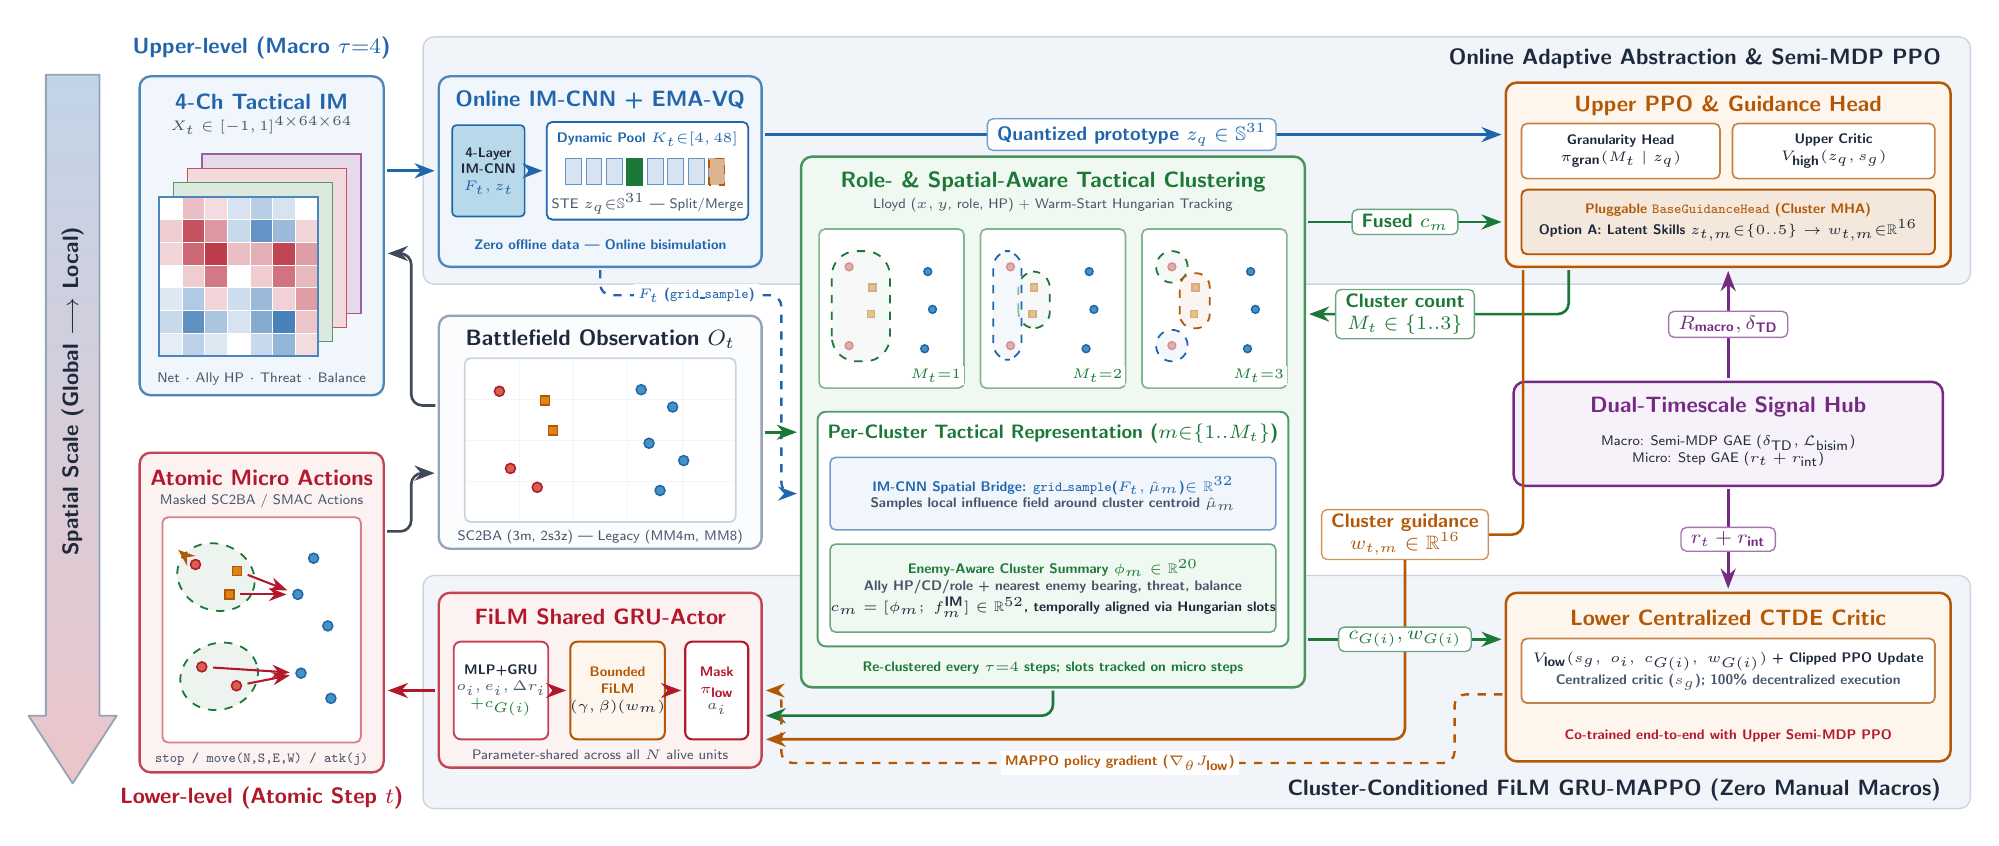
\begin{tikzpicture}[
  x=1cm, y=1cm,
  >=Stealth,
  font=\sffamily\footnotesize,
  selfdot/.style={circle, fill=cRedMid, draw=cRed, line width=0.55pt, inner sep=0pt, minimum size=3.6pt},
  meleedot/.style={regular polygon, regular polygon sides=4, fill=cOrangeMid, draw=cOrange, line width=0.55pt, inner sep=0pt, minimum size=4.6pt},
  enemydot/.style={circle, fill=cBlueMid, draw=cBlue, line width=0.55pt, inner sep=0pt, minimum size=3.6pt},
  flow/.style={->, line width=0.95pt, draw=cInk!85, shorten >=1.5pt, shorten <=1.2pt},
  flowcol/.style={->, line width=0.95pt, draw=#1, shorten >=1.5pt, shorten <=1.2pt},
  dashcol/.style={->, dashed, line width=0.85pt, draw=#1, shorten >=1.5pt, shorten <=1.2pt},
  edgelbl/.style={
    rectangle, rounded corners=2pt, fill=white, draw=#1!65,
    line width=0.5pt, font=\sffamily\scriptsize\bfseries, text=#1,
    inner xsep=3.5pt, inner ysep=1.6pt
  }
]

% =====================================================================
% 0. Subtle Upper-level (Slow Macro) & Lower-level (Fast Micro) Bands
% =====================================================================
\begin{scope}[on background layer]
  \filldraw[fill=cBand, draw=cLine, rounded corners=4pt, line width=0.5pt]
    (4.95, 6.86) rectangle (24.60, 10.00);
  \filldraw[fill=cBand, draw=cLine, rounded corners=4pt, line width=0.5pt]
    (4.95, 0.20) rectangle (24.60, 3.16);
\end{scope}

\node[font=\sffamily\footnotesize\bfseries\itshape, text=cBlue] at (2.90, 9.86) {Upper-level (Macro $\tau{=}4$)};
\node[font=\sffamily\footnotesize\bfseries\itshape, text=cRed]  at (2.90, 0.34) {Lower-level (Atomic Step $t$)};
\node[font=\sffamily\footnotesize\bfseries\itshape, text=cInk, anchor=east] at (24.35, 9.72) {Online Adaptive Abstraction \& Semi-MDP PPO};
\node[font=\sffamily\footnotesize\bfseries\itshape, text=cInk, anchor=east] at (24.35, 0.44) {Cluster-Conditioned FiLM GRU-MAPPO (Zero Manual Macros)};

% =====================================================================
% 1. Leftmost Spatial Scale Gradient Arrow
% =====================================================================
\shade[top color=cBlue!28, bottom color=cRed!25, draw=cGray, line width=0.65pt, line join=round]
  (0.16, 9.52) -- (0.84, 9.52) -- (0.84, 1.38) -- (1.06, 1.38) -- (0.50, 0.52) -- (-0.06, 1.38) -- (0.16, 1.38) -- cycle;
\node[font=\sffamily\footnotesize\bfseries, text=cInk, rotate=90] at (0.50, 5.50) {Spatial Scale (Global $\longrightarrow$ Local)};

% =====================================================================
% 2. Column 1 (x=1.35..4.45): 4-Ch Tactical IM & Atomic Actions
% =====================================================================
\filldraw[fill=cBlueBg, draw=cBlue!80, rounded corners=4pt, line width=0.85pt]
  (1.35, 5.45) rectangle (4.45, 9.50);
\node[font=\sffamily\footnotesize\bfseries, text=cBlue] at (2.90, 9.18) {4-Ch Tactical IM};
\node[font=\sffamily\tiny, text=cMuted] at (2.90, 8.88) {$X_t \in [-1,1]^{4\times 64\times 64}$};

\begin{scope}[shift={(1.60, 5.95)}]
  \filldraw[fill=cPurple!18, draw=cPurple!75, line width=0.55pt] (0.54, 0.54) rectangle ++(2.02, 2.02);
  \filldraw[fill=cRed!16, draw=cRed!75, line width=0.55pt] (0.36, 0.36) rectangle ++(2.02, 2.02);
  \filldraw[fill=cGreen!16, draw=cGreen!75, line width=0.55pt] (0.18, 0.18) rectangle ++(2.02, 2.02);
  \fill[white] (0,0) rectangle (2.02, 2.02);
  \foreach \r/\c/\col in {
    0/0/cBlue!12, 0/1/cBlue!30, 0/2/cBlue!15, 0/3/white,    0/4/cBlue!25, 0/5/cBlue!48, 0/6/cRed!15,
    1/0/cBlue!25, 1/1/cBlue!72, 1/2/cBlue!38, 1/3/cBlue!18, 1/4/cBlue!55, 1/5/cBlue!82, 1/6/cRed!25,
    2/0/cBlue!15, 2/1/cBlue!35, 2/2/cRed!18,  2/3/cBlue!22, 2/4/cBlue!45, 2/5/cRed!20,  2/6/cRed!42,
    3/0/white,    3/1/cRed!22,  3/2/cRed!58,  3/3/white,    3/4/cRed!22,  3/5/cRed!60,  3/6/cRed!30,
    4/0/cRed!18,  4/1/cRed!65,  4/2/cRed!85,  4/3/cRed!28,  4/4/cRed!35,  4/5/cRed!80,  4/6/cRed!42,
    5/0/cRed!22,  5/1/cRed!75,  5/2/cRed!45,  5/3/cBlue!25, 5/4/cBlue!70, 5/5/cBlue!45, 5/6/cRed!18,
    6/0/white,    6/1/cRed!28,  6/2/cRed!15,  6/3/cBlue!18, 6/4/cBlue!32, 6/5/cBlue!18, 6/6/white%
  }{
    \fill[\col] (\c*0.288, \r*0.288) rectangle ++(0.288, 0.288);
  }
  \foreach \x in {0,...,7} {\draw[white, line width=0.3pt] (\x*0.288, 0) -- (\x*0.288, 2.02);}
  \foreach \y in {0,...,7} {\draw[white, line width=0.3pt] (0, \y*0.288) -- (2.02, \y*0.288);}
  \draw[cBlue!80, line width=0.65pt] (0,0) rectangle (2.02, 2.02);
\end{scope}
\node[font=\sffamily\tiny, text=cMuted] at (2.90, 5.66) {Net $\cdot$ Ally HP $\cdot$ Threat $\cdot$ Balance};

\filldraw[fill=cRedBg, draw=cRed!80, rounded corners=4pt, line width=0.85pt]
  (1.35, 0.66) rectangle (4.45, 4.72);
\node[font=\sffamily\footnotesize\bfseries, text=cRed] at (2.90, 4.40) {Atomic Micro Actions};
\node[font=\sffamily\tiny, text=cMuted] at (2.90, 4.10) {Masked SC2BA / SMAC Actions};

\begin{scope}[shift={(1.64, 1.04)}]
  \filldraw[fill=white, draw=cRed!55, rounded corners=2pt, line width=0.65pt] (0,0) rectangle (2.52, 2.86);
  \draw[cGreen, fill=cGreen!8, dashed, line width=0.65pt, rotate around={-20:(0.68,2.10)}] (0.68,2.10) ellipse (0.50cm and 0.42cm);
  \draw[cGreen, fill=cGreen!8, dashed, line width=0.65pt, rotate around={18:(0.72,0.84)}] (0.72,0.84) ellipse (0.50cm and 0.42cm);
  \node[meleedot] (maS1) at (0.95, 2.18) {};
  \node[meleedot] (maS2) at (0.85, 1.88) {};
  \node[selfdot]  (maS3) at (0.42, 2.26) {};
  \node[selfdot]  (maS4) at (0.50, 0.96) {};
  \node[selfdot]  (maS5) at (0.94, 0.72) {};
  \node[enemydot] (maE1) at (1.92, 2.34) {};
  \node[enemydot] (maE2) at (1.72, 1.88) {};
  \node[enemydot] (maE3) at (2.10, 1.48) {};
  \node[enemydot] (maE4) at (1.76, 0.88) {};
  \node[enemydot] (maE5) at (2.14, 0.56) {};
  \draw[->, cRed, line width=0.75pt, shorten >=2pt, shorten <=2pt] (maS1) -- (maE2);
  \draw[->, cRed, line width=0.75pt, shorten >=2pt, shorten <=2pt] (maS2) -- (maE2);
  \draw[->, cOrange, line width=0.70pt, shorten >=1.5pt, shorten <=2pt] (maS3) -- (0.16, 2.48);
  \draw[->, cRed, line width=0.75pt, shorten >=2pt, shorten <=2pt] (maS4) -- (maE4);
  \draw[->, cRed, line width=0.75pt, shorten >=2pt, shorten <=2pt] (maS5) -- (maE4);
\end{scope}
\node[font=\sffamily\tiny, text=cMuted] at (2.90, 0.83) {\texttt{stop / move(N,S,E,W) / atk(j)}};

% =====================================================================
% 3. Column 2 (x=5.15..9.25): Online IM-CNN+VQ, Obs, FiLM Actor
% =====================================================================
\filldraw[fill=cBlueBg, draw=cBlue!80, rounded corners=4pt, line width=0.85pt]
  (5.15, 7.08) rectangle (9.25, 9.50);
\node[font=\sffamily\footnotesize\bfseries, text=cBlue] at (7.20, 9.20) {Online IM-CNN + EMA-VQ};
\filldraw[fill=cBlueLt!65, draw=cBlue, rounded corners=1.5pt, line width=0.6pt] (5.32, 7.72) rectangle (6.24, 8.88);
\node[font=\sffamily\tiny\bfseries, text=cInk, align=center] at (5.78, 8.30) {4-Layer\\IM-CNN\\{\color{cBlue}$F_t, z_t$}};
\draw[flowcol=cBlue] (6.24, 8.30) -- (6.52, 8.30);
\filldraw[fill=white, draw=cBlue, rounded corners=2pt, line width=0.65pt] (6.52, 7.68) rectangle (9.08, 8.92);
\node[font=\sffamily\tiny\bfseries, text=cBlue] at (7.80, 8.70) {Dynamic Pool $K_t{\in}[4,48]$};
\begin{scope}[shift={(6.76, 8.12)}]
  \foreach \k in {0,...,7} {
    \filldraw[fill=cBlue!18, draw=cBlue!70, line width=0.38pt] (\k*0.26, 0) rectangle ++(0.20, 0.34);
  }
  \filldraw[fill=cGreen, draw=cGreen, line width=0.45pt] (3*0.26, 0) rectangle ++(0.20, 0.34);
  \filldraw[fill=cOrange!45, draw=cOrange, dashed, line width=0.45pt] (7*0.26, 0) rectangle ++(0.20, 0.34);
\end{scope}
\node[font=\sffamily\tiny, text=cMuted] at (7.80, 7.88) {STE $z_q{\in}\mathbb{S}^{31}$ | Split/Merge};
\node[font=\sffamily\tiny\bfseries, text=cBlue] at (7.20, 7.36) {Zero offline data | Online bisimulation};

% Observation card
\filldraw[fill=cPanel, draw=cGray, rounded corners=4pt, line width=0.85pt]
  (5.15, 3.50) rectangle (9.25, 6.46);
\node[font=\sffamily\footnotesize\bfseries, text=cInk] at (7.20, 6.16) {Battlefield Observation $O_t$};
\begin{scope}[shift={(5.48, 3.84)}]
  \filldraw[fill=white, draw=cLine, rounded corners=2pt, line width=0.65pt] (0,0) rectangle (3.44, 2.08);
  \foreach \gx in {0.69, 1.38, 2.07, 2.76} {\draw[cBand, line width=0.35pt] (\gx, 0.02) -- (\gx, 2.06);}
  \foreach \gy in {0.52, 1.04, 1.56} {\draw[cBand, line width=0.35pt] (0.02, \gy) -- (3.42, \gy);}
  \foreach \ux/\uy in {0.44/1.66, 0.58/0.68, 0.92/0.44} {\node[selfdot] at (\ux,\uy) {};}
  \foreach \ux/\uy in {1.02/1.54, 1.12/1.16} {\node[meleedot] at (\ux,\uy) {};}
  \foreach \ux/\uy in {2.24/1.68, 2.64/1.46, 2.34/1.00, 2.78/0.78, 2.48/0.40} {\node[enemydot] at (\ux,\uy) {};}
\end{scope}
\node[font=\sffamily\tiny, text=cMuted] at (7.20, 3.65) {SC2BA (3m, 2s3z) | Legacy (MM4m, MM8)};

% FiLM Shared GRU-Actor card
\filldraw[fill=cRedBg, draw=cRed!80, rounded corners=4pt, line width=0.85pt]
  (5.15, 0.72) rectangle (9.25, 2.94);
\node[font=\sffamily\footnotesize\bfseries, text=cRed] at (7.20, 2.64) {FiLM Shared GRU-Actor};
\filldraw[fill=white, draw=cRed!80, rounded corners=2.5pt, line width=0.7pt] (5.34, 1.08) rectangle (6.54, 2.32);
\node[font=\sffamily\tiny\bfseries, text=cInk, align=center] at (5.94, 1.70) {MLP+GRU\\{\color{cMuted}$o_i, e_i, \Delta r_i$}\\{\color{cGreen}$+ c_{G(i)}$}};
\draw[flowcol=cRed] (6.54, 1.70) -- (6.82, 1.70);
\filldraw[fill=cOrangeBg, draw=cOrange, rounded corners=2.5pt, line width=0.75pt] (6.82, 1.08) rectangle (8.02, 2.32);
\node[font=\sffamily\tiny\bfseries, text=cOrange, align=center] at (7.42, 1.70) {Bounded\\FiLM\\{\color{cInk}$(\gamma,\beta)(w_m)$}};
\draw[flowcol=cRed] (8.02, 1.70) -- (8.28, 1.70);
\filldraw[fill=white, draw=cRed, rounded corners=2.5pt, line width=0.75pt] (8.28, 1.08) rectangle (9.08, 2.32);
\node[font=\sffamily\tiny\bfseries, text=cRed, align=center] at (8.68, 1.70) {Mask\\$\pi_{\text{low}}$\\{\color{cMuted}$a_i$}};
\node[font=\sffamily\tiny, text=cMuted] at (7.20, 0.88) {Parameter-shared across all $N$ alive units};

% =====================================================================
% 4. Column 3 (x=9.75..16.15): Role/Spatial Tactical Clustering Hub
% =====================================================================
\filldraw[fill=cGreenBg, draw=cGreen!80, rounded corners=4pt, line width=0.9pt]
  (9.75, 1.74) rectangle (16.15, 8.48);
\node[font=\sffamily\footnotesize\bfseries, text=cGreen] at (12.95, 8.16) {Role- \& Spatial-Aware Tactical Clustering};
\node[font=\sffamily\tiny, text=cMuted] at (12.95, 7.86) {Lloyd ($x,y$, role, HP) + Warm-Start Hungarian Tracking};

\newcommand{\clustermini}[3]{%
  \begin{scope}[shift={(#1, #2)}]
    \filldraw[fill=white, draw=cGreen!55, rounded corners=2pt, line width=0.6pt] (0,0) rectangle (1.84, 2.02);
    \node[selfdot, minimum size=2.8pt] at (0.38, 1.54) {};
    \node[meleedot, minimum size=3.6pt] at (0.68, 1.28) {};
    \node[meleedot, minimum size=3.6pt] at (0.66, 0.94) {};
    \node[selfdot, minimum size=2.8pt] at (0.38, 0.54) {};
    \node[enemydot, minimum size=2.8pt] at (1.38, 1.48) {};
    \node[enemydot, minimum size=2.8pt] at (1.44, 1.00) {};
    \node[enemydot, minimum size=2.8pt] at (1.34, 0.50) {};
    \node[font=\sffamily\tiny\bfseries, text=cGreen, fill=white, inner sep=1pt] at (1.48, 0.16) {#3};
  \end{scope}
}

\clustermini{9.98}{5.54}{$M_t{=}1$}
\begin{scope}[shift={(9.98, 5.54)}]
  \draw[cGreen, fill=cGreen!8, fill opacity=0.55, dashed, rounded corners=9pt, line width=0.65pt]
    (0.16, 0.34) rectangle (0.90, 1.74);
\end{scope}
\clustermini{12.03}{5.54}{$M_t{=}2$}
\begin{scope}[shift={(12.03, 5.54)}]
  \draw[cGreen, fill=cGreen!8, fill opacity=0.55, dashed, rounded corners=6pt, line width=0.65pt]
    (0.48, 0.76) rectangle (0.88, 1.48);
  \draw[cBlue, fill=cBlue!8, fill opacity=0.55, dashed, rounded corners=6pt, line width=0.65pt]
    (0.16, 0.36) rectangle (0.52, 1.74);
\end{scope}
\clustermini{14.08}{5.54}{$M_t{=}3$}
\begin{scope}[shift={(14.08, 5.54)}]
  \draw[cGreen, fill=cGreen!8, fill opacity=0.55, dashed, line width=0.65pt] (0.38, 1.54) circle (0.20cm);
  \draw[cOrange, fill=cOrange!10, fill opacity=0.55, dashed, rounded corners=5pt, line width=0.65pt]
    (0.48, 0.76) rectangle (0.86, 1.46);
  \draw[cBlue, fill=cBlue!8, fill opacity=0.55, dashed, line width=0.65pt] (0.38, 0.54) circle (0.20cm);
\end{scope}

% Per-cluster representation card with generous interior margins
\filldraw[fill=white, draw=cGreen!75, rounded corners=3pt, line width=0.7pt]
  (9.96, 2.26) rectangle (15.94, 5.24);
\node[font=\sffamily\scriptsize\bfseries, text=cGreen] at (12.95, 4.96) {Per-Cluster Tactical Representation ($m{\in}\{1..M_t\}$)};

\filldraw[fill=cBlueBg, draw=cBlue!65, rounded corners=2pt, line width=0.55pt] (10.12, 3.74) rectangle (15.78, 4.66);
\node[font=\sffamily\tiny\bfseries, text=cBlue, align=center] at (12.95, 4.20)
  {IM-CNN Spatial Bridge: \texttt{grid\_sample}($F_t, \hat{\mu}_m$)$\in\mathbb{R}^{32}$\\
   {\color{cMuted}Samples local influence field around cluster centroid $\hat{\mu}_m$}};

\filldraw[fill=cGreenBg, draw=cGreen!65, rounded corners=2pt, line width=0.55pt] (10.12, 2.44) rectangle (15.78, 3.56);
\node[font=\sffamily\tiny\bfseries, text=cGreen, align=center] at (12.95, 3.00)
  {Enemy-Aware Cluster Summary $\phi_m \in \mathbb{R}^{20}$\\
   {\color{cMuted}Ally HP/CD/role + nearest enemy bearing, threat, balance}\\
   {\color{cInk}$c_m = [\phi_m;\; f^{\text{IM}}_m] \in \mathbb{R}^{52}$, temporally aligned via Hungarian slots}};

\node[font=\sffamily\tiny\bfseries, text=cGreen] at (12.95, 1.98) {Re-clustered every $\tau{=}4$ steps; slots tracked on micro steps};

% =====================================================================
% 5. Column 4 (x=18.70..24.35): Upper Guidance PPO, Reward Hub, Lower Critic
% =====================================================================
\filldraw[fill=cOrangeBg, draw=cOrange, rounded corners=4pt, line width=0.9pt]
  (18.70, 7.08) rectangle (24.35, 9.42);
\node[font=\sffamily\footnotesize\bfseries, text=cOrange] at (21.525, 9.12) {Upper PPO \& Guidance Head};
\filldraw[fill=white, draw=cOrange!75, rounded corners=2pt, line width=0.6pt] (18.90, 8.20) rectangle (21.42, 8.90);
\node[font=\sffamily\tiny\bfseries, text=cInk, align=center] at (20.16, 8.55) {Granularity Head\\$\pi_{\text{gran}}(M_t \mid z_q)$};
\filldraw[fill=white, draw=cOrange!75, rounded corners=2pt, line width=0.6pt] (21.58, 8.20) rectangle (24.15, 8.90);
\node[font=\sffamily\tiny\bfseries, text=cInk, align=center] at (22.865, 8.55) {Upper Critic\\$V_{\text{high}}(z_q, s_g)$};
\filldraw[fill=cOrange!14, draw=cOrange, rounded corners=2pt, line width=0.7pt] (18.90, 7.24) rectangle (24.15, 8.06);
\node[font=\sffamily\tiny\bfseries, text=cOrange, align=center] at (21.525, 7.65)
  {Pluggable \texttt{BaseGuidanceHead} (Cluster MHA)\\
   {\color{cInk}Option A: Latent Skills $z_{t,m}{\in}\{0..5\} \to w_{t,m}{\in}\mathbb{R}^{16}$}};

% Dual-Timescale Signal Hub (wider with clean 2-line wrap)
\filldraw[fill=cPurpleBg, draw=cPurple, rounded corners=4pt, line width=0.9pt]
  (18.80, 4.30) rectangle (24.25, 5.62);
\node[font=\sffamily\footnotesize\bfseries, text=cPurple] at (21.525, 5.30) {Dual-Timescale Signal Hub};
\node[font=\sffamily\tiny, text=cInk, align=center] at (21.525, 4.74)
  {Macro: Semi-MDP GAE ($\delta_{\text{TD}}, \mathcal{L}_{\text{bisim}}$)\\
   Micro: Step GAE ($r_t + r_{\text{int}}$)};

% Lower Centralized CTDE Critic
\filldraw[fill=cOrangeBg, draw=cOrange, rounded corners=4pt, line width=0.9pt]
  (18.70, 0.80) rectangle (24.35, 2.94);
\node[font=\sffamily\footnotesize\bfseries, text=cOrange] at (21.525, 2.62) {Lower Centralized CTDE Critic};
\filldraw[fill=white, draw=cOrange!75, rounded corners=2pt, line width=0.65pt] (18.90, 1.54) rectangle (24.15, 2.36);
\node[font=\sffamily\tiny\bfseries, text=cInk, align=center] at (21.525, 1.95)
  {$V_{\text{low}}(s_g,\; o_i,\; c_{G(i)},\; w_{G(i)})$ + Clipped PPO Update\\
   {\color{cMuted}Centralized critic ($s_g$); 100\% decentralized execution}};
\node[font=\sffamily\tiny\bfseries, text=cRed] at (21.525, 1.12) {Co-trained end-to-end with Upper Semi-MDP PPO};

% =====================================================================
% 6. Clean Non-Overlapping Orthogonal Signal Arrows
% =====================================================================
\draw[flow, rounded corners=4pt] (5.15, 5.32) -- (4.80, 5.32) -- (4.80, 7.25) -- (4.45, 7.25);
\draw[flowcol=cBlue] (4.45, 8.30) -- (5.15, 8.30);

% z_q -> Upper PPO
\draw[flowcol=cBlue, rounded corners=3pt] (9.25, 8.76) -- (18.70, 8.76);
\node[edgelbl=cBlue] at (13.95, 8.76) {Quantized prototype $z_q \in \mathbb{S}^{31}$};

% F_t spatial bridge -> Tactical Clustering
\draw[dashcol=cBlue, rounded corners=4pt] (7.20, 7.08) -- (7.20, 6.72) -- (9.50, 6.72) -- (9.50, 4.20) -- (9.75, 4.20);
\node[font=\sffamily\tiny\bfseries, text=cBlue, fill=white, inner sep=1.5pt] at (8.42, 6.72) {$F_t$ (\texttt{grid\_sample})};

% Observation -> Clustering
\draw[flowcol=cGreen] (9.25, 4.98) -- (9.75, 4.98);

% Upper Granularity M_t -> Clustering
\draw[flowcol=cGreen, rounded corners=4pt] (19.50, 7.08) -- (19.50, 6.48) -- (16.15, 6.48);
\node[edgelbl=cGreen, align=center] at (17.42, 6.48) {Cluster count\\$M_t \in \{1..3\}$};

% Clustering c_m -> Upper Guidance Head
\draw[flowcol=cGreen] (16.15, 7.65) -- (18.70, 7.65);
\node[edgelbl=cGreen] at (17.42, 7.65) {Fused $c_m$};

% Upper Guidance w_{t,m} -> Lower FiLM Actor (routed cleanly BELOW green hub at y=1.08!)
\draw[flowcol=cOrange, rounded corners=4pt] (18.92, 7.08) -- (18.92, 3.68) -- (17.42, 3.68) -- (17.42, 1.08) -- (9.25, 1.08);
\node[edgelbl=cOrange, align=center] at (17.42, 3.68) {Cluster guidance\\$w_{t,m} \in \mathbb{R}^{16}$};

% Clustering -> Lower Critic (c_{G(i)}, w_{G(i)}) & -> FiLM Actor (at y=1.34)
\draw[flowcol=cGreen] (16.15, 2.35) -- (18.70, 2.35);
\node[edgelbl=cGreen] at (17.42, 2.35) {$c_{G(i)}, w_{G(i)}$};
\draw[flowcol=cGreen, rounded corners=4pt] (12.95, 1.74) -- (12.95, 1.38) -- (9.25, 1.38);

% Lower Critic PPO gradient -> FiLM Actor (routed cleanly in bottom corridor y=0.78!)
\draw[dashcol=cOrange, rounded corners=4pt] (18.70, 1.65) -- (18.05, 1.65) -- (18.05, 0.78) -- (9.50, 0.78) -- (9.50, 1.70) -- (9.25, 1.70);
\node[font=\sffamily\tiny\bfseries, text=cOrange, fill=white, inner sep=1.5pt] at (13.80, 0.78) {MAPPO policy gradient ($\nabla_\theta J_{\text{low}}$)};

% Signal Hub -> Upper & Lower
\draw[flowcol=cPurple] (21.525, 5.62) -- (21.525, 7.08);
\node[edgelbl=cPurple] at (21.525, 6.35) {$R_{\text{macro}}, \delta_{\text{TD}}$};
\draw[flowcol=cPurple] (21.525, 4.30) -- (21.525, 2.94);
\node[edgelbl=cPurple] at (21.525, 3.62) {$r_t + r_{\text{int}}$};

% FiLM Actor -> Micro Actions -> Observation
\draw[flowcol=cRed] (5.15, 1.70) -- (4.45, 1.70);
\draw[flow, rounded corners=4pt] (4.45, 3.72) -- (4.80, 3.72) -- (4.80, 4.46) -- (5.15, 4.46);

\end{tikzpicture}
\end{document}
